%!TEX root = ../main.tex
\begin{frame}{Toy example and classic vaccination OC}
    \setlength{\leftmargini}{1mm}
    \begin{textblock*}{65mm}(0mm, 18mm)
        \only<1->{
            To fix ideas:
            \begin{equation*}
                \begin{aligned}
                    S'(t) &= -\beta IS
                    \\
                    I'(t) &=  \beta IS - \gamma I
                    \\
                    R'(t) & = \gamma I
                    \\
                    & S(0) = S_0, I(0)=I_0, R(0)=0
                    \\
                    & S(t) + I(t) + R(t )= 1
                \end{aligned}
            \end{equation*}
        }
    \end{textblock*}
%     %
    \begin{textblock*}{65mm}(65mm, 18mm)
        \only<2>{
            With vaccination
            \begin{equation*}
                \begin{aligned}
                    S'(t) &= -\beta IS  - \textcolor{red}{\lambda_V(t)}
                    \\
                    I'(t) &=  \beta IS - \gamma I
                    \\
                    R'(t) & = \gamma I
                    \\
                    V'(t) & = \textcolor{red}{\lambda_V(t)}
                    \\
                    & S(0) = S_0, I(0)=I_0,
                    \\
                    &R(0)=0, V(0) = 0
                    \\
                    & S(t) + I(t) + R(t) + V(t)= 1
                \end{aligned}
            \end{equation*}
        }
    \end{textblock*}
    \begin{textblock*}{65mm}(65mm, 18mm)
        \only<3->{
            \begin{equation*}
                \begin{aligned}
                    S'(t) &= -\beta IS  - \textcolor{red}{\lambda_V(x, t)}
                    \\
                    I'(t) &=  \beta IS - \gamma I
                    \\
                    R'(t) & = \gamma I
                    \\
                    V'(t) & = \textcolor{red}{\lambda_V(x,t)}
                \end{aligned}
            \end{equation*}
        }
    \end{textblock*}
    \begin{textblock*}{28mm}(5mm, 50mm)
        \begin{block}{``Classic'' Vaccination}
            \begin{itemize}
                \item
                \only<4->{
                    Gumel,
                }
                \only<6->{
                    $$
                    \lambda_V:=
                    \underbrace{ \textcolor{orange}{\xi}}_{cte.}
                    \cdot \ S(t)
                    $$
                }

            \end{itemize}
            \only<7->{
                Optimal Controlled:
            }
        \end{block}
    \end{textblock*}
    \begin{textblock*}{80mm}(45mm,48mm)
            \only<6>{
                \begin{bibunit}[apalike]
                    \nocite{Alexander2004,Iboi2020}
                    \putbib
                \end{bibunit}
            }
            \only<7>{
                \begin{bibunit}[apalike]
                    \nocite{Hethcote1973,Wickwire1977}
                    \putbib
                \end{bibunit}
            }
    \end{textblock*}
 \end{frame}
% %%%%%%%%%%%%%%%%%%%%%%%%%%%%%%%%%%%%%%%%%%%%%%%%%%%%%%%%%%%%%%%%%%%%%%%%%%%%%%
\begin{frame}{The Basic Optimization Question}
    \begin{textblock*}{72.5mm}(0mm, 10mm)
        \begin{graybox}{Hypothesis}
            \only<1->{
                \textbf{Cost:}
                The \textbf{effort} expended in
                ``\textbf{preventing-mitigating}
                an epidemic'' by vaccination is
                \textbf{proportional} to the vaccination
                rate $\lambda_V$.\\
            }
%            %
            \only<2->{
                \textbf{Jabs Counter:}
                If $S(0)\approx 1$ , $X(\cdot):$ counts
                vaccine doses, then
                $$
                X(t) = 1 - \exp(-\lambda_V t),
                $$
                estimates the fraction of vaccinated
                individuals.
                Thus, for time horizon $T$ and
                vaccination coverage %$X_{cov}$
            }
            \only<3-6>{
                \begin{equation*}
                    \begin{aligned}
                        X_{cov} &= X(T)
                        \\
                        &\approx
                        1 - \exp(-\textcolor{teal}{\lambda_V} T).
                    \end{aligned}
                \end{equation*}
            }
        \end{graybox}
    \end{textblock*}
    \begin{textblock*}{50mm}(75mm, 10mm)
        \only<4->{
            \begin{yellowbox}{{Given $X_{cov}$, \ $T$}}
                $$
                \lambda_V = -\frac{1}{T}
                \ln(1 - X_{cov})
                $$
                \textbf{estimates} the constant vaccination rate s.t.,
                afther time $T$, we reach $X_{cov}$.
            \end{yellowbox}
        }
        \only<5->{
            \begin{greenbox}{{$X_{COV}: 70 \%$, $T$: one \SI{}{year}}}
                $
                \lambda_V \approx \num{0.00329}
                $
                \tcblower
                \only<6>{
                    If $S(0) N$ corresponds to HMS
                    (\SI{812229}{inhabitants})
                    $
                    % \num{0.00611352} \times \num{100000}
                    \approx \SI{2668}{jabs \per day}.
                    $
                }
                \only<7->{
                    \textcolor{orange}{
                        \textbf{
                            How to optimize vaccination?}
                    }
                }
            \end{greenbox}
        }
    \end{textblock*}
%     %--------------------------------------------------------------------------
    \setbeamertemplate{itemize items}[ball]
    \begin{textblock*}{62mm}(5mm, 70mm)
        \only<8->{
            \begin{block}{Common Objectives}
                \begin{itemize}
                    \item
                    \only<9->{

                        Who to vaccine first?
                        (Allocation)
                    }
                    \item
                    \only<10->{

                        How and when?
                        (Administration)
                    }
                \end{itemize}
            \end{block}
        }
    \end{textblock*}
\end{frame}
%%%%%%%%%%%%%%%%%%%%%%%%%%%%%%%%%%%%%%%%%%%%%%%%%%%%%%%%%%%%%%%%%%%%%%%%%%%%%%%%
 \begin{frame}{Vaccine optimiztion for COVID-19}
    \begin{textblock*}{40mm}(5mm, 15mm)
        \setbeamertemplate{itemize items}[ball]
        \begin{block}{Common Objectives}
             \begin{itemize}%
                 \item
                 \textcolor<5>{orange}{
                     Who to vaccine first?
                     (Allocation)
                 }
                 \only<2->{
                     \item
                     \textcolor<6->{orange}{
                         How and when?
                         \textbf<7>{
                             (Administration)
                         }
                     }
                 }
             \end{itemize}
         \end{block}
    \end{textblock*}
%     %
    \begin{textblock*}{65mm}(55mm, 15mm)
        \only<2->{
            \begin{block}{%
                    \only<2-3>{Cost}
                    \only<4->{Optimal Control Problem}
                }
                \only<3>{
                    \begin{equation*}
                        \begin{aligned}
                            % \min_{\mathbf{u} \in \mathcal{U}}
                            J(u) := &
                            \varphi(x(T)) +
                            \int_0 ^  T
                            f(t, x(t), u(t))
                        \end{aligned}
                    \end{equation*}
                }
                \only<4->{
                    \begin{equation*}
                        \begin{aligned}
                            \min_{\mathbf{u} \in \mathcal{U}}
                            J(u) = &
                            \varphi(x(T)) +
                            \int_0 ^  T
                            f(t, x(t), u(t))
                            \\
                            \dot{x}(t) =& b(t,u(t), x(t)),
                            \quad \text{a.e. }t \in[0,T].
                        \end{aligned}
                    \end{equation*}
                }
            \end{block}
        }
    \end{textblock*}
%     %
    \begin{textblock*}{115mm}(10mm, 42mm)
        \only<5>{
            \begin{bibunit}[apalike]
                \nocite{Matrajt2020,Bubar2020}
                \putbib
            \end{bibunit}
        }
        \only<6-7>{
            \begin{bibunit}[apalike]
                \nocite{Zegarra2020, Salcedo-Varela2021}
                \putbib
            \end{bibunit}
        }
    \end{textblock*}
\end{frame}
%
%
%
\begin{frame}{Setup}
        \begin{textblock*}{120mm}(0mm,10mm)
            \begin{overlayarea}{\textwidth}{\textheight}
                \begin{center}
                \only<1>{
                    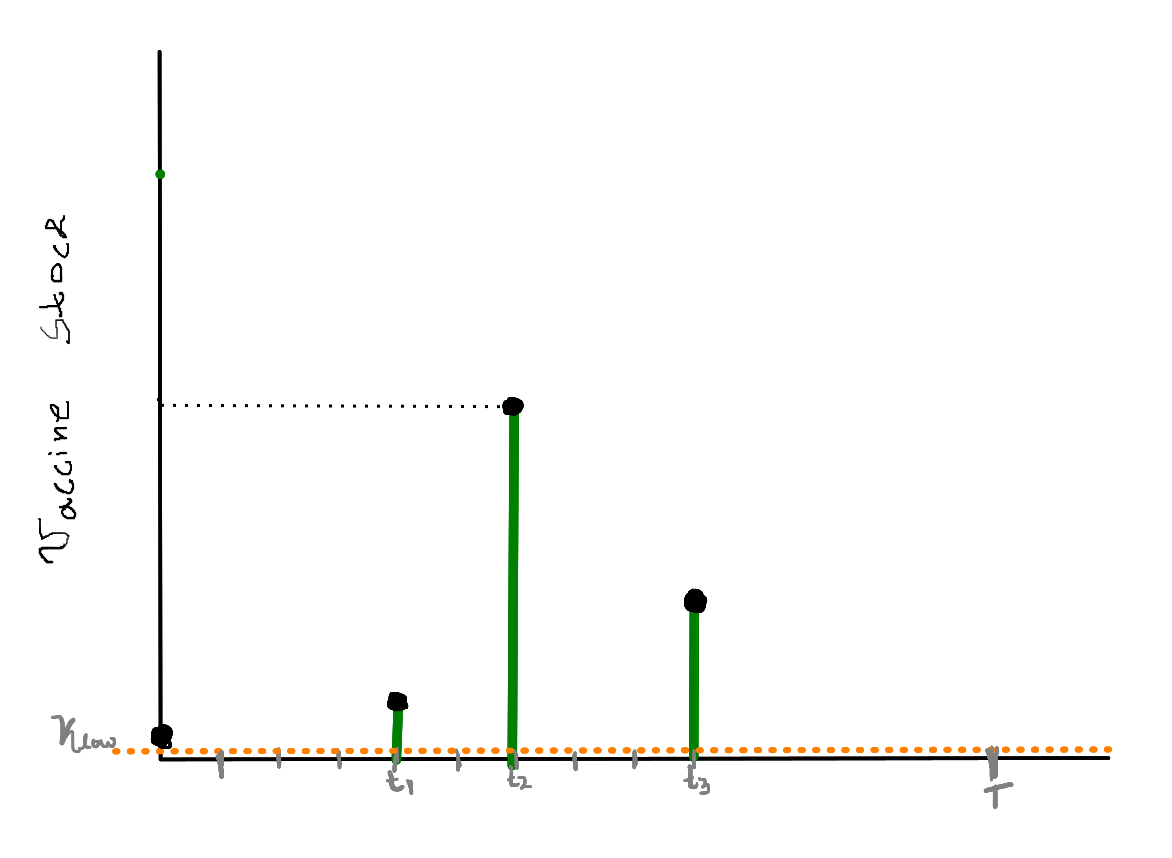
\includegraphics[%
                        width=\textwidth,%
                        keepaspectratio=true]{images/Fig01_000.png}
                }
                \only<2>{
                    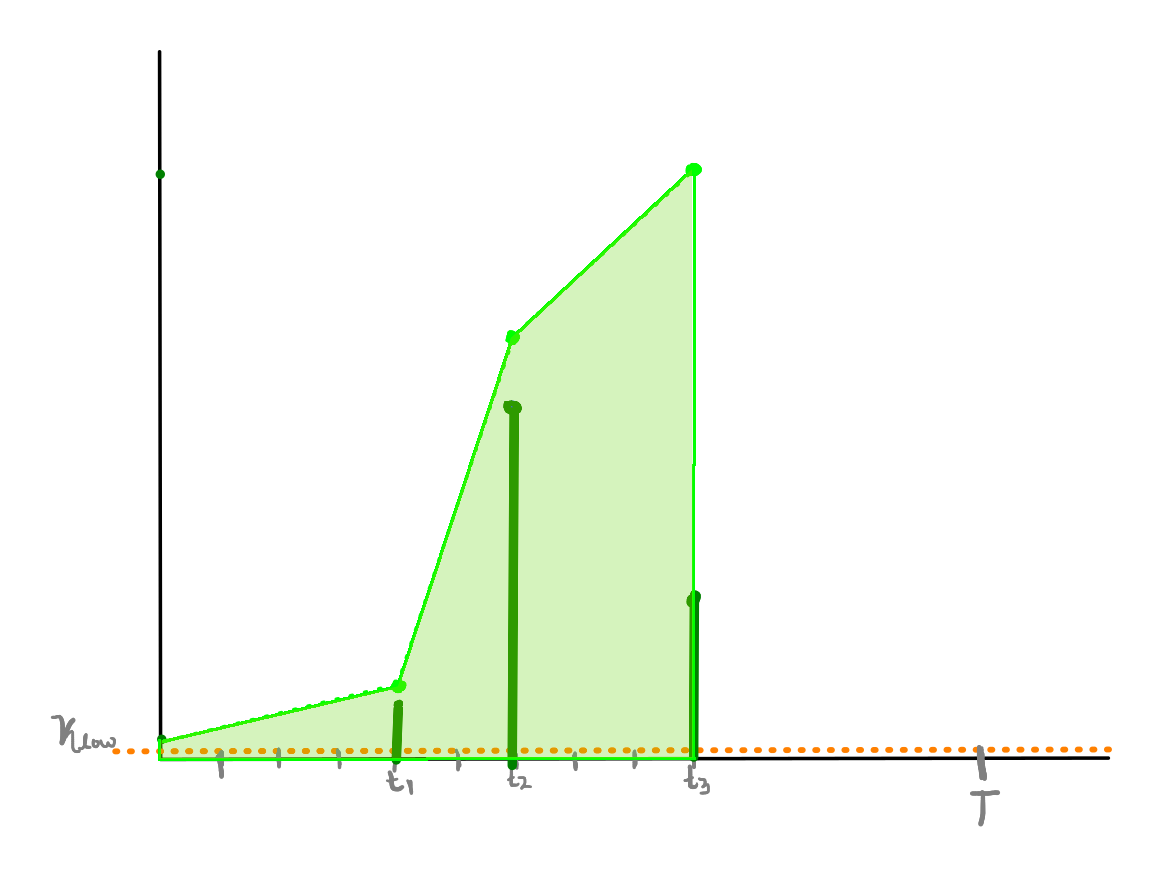
\includegraphics[%
                        width=\textwidth,%
                        keepaspectratio=true]{images/Fig01_001.png}
                }
                \only<3>{
                    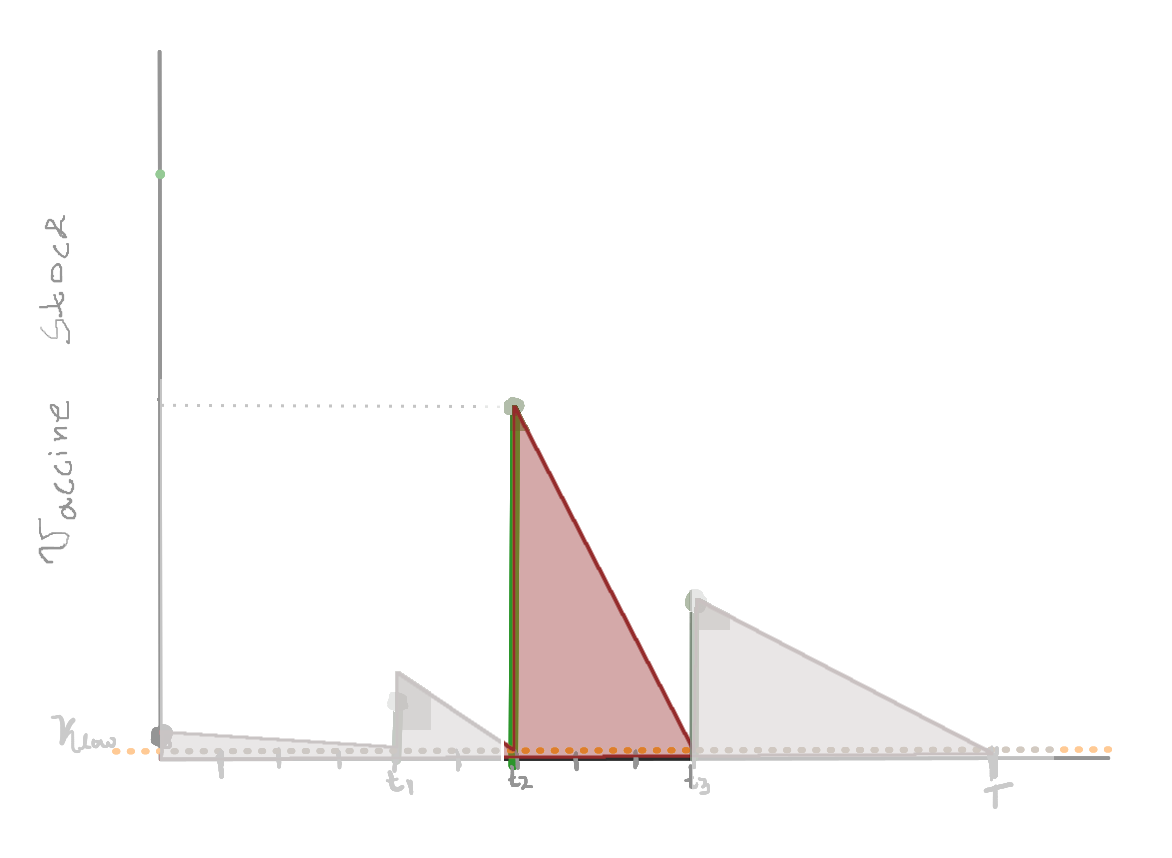
\includegraphics[%
                        width=\textwidth,%
                        keepaspectratio=true]{images/Fig01_002_00.png}
                }

                \only<4-5>{
                    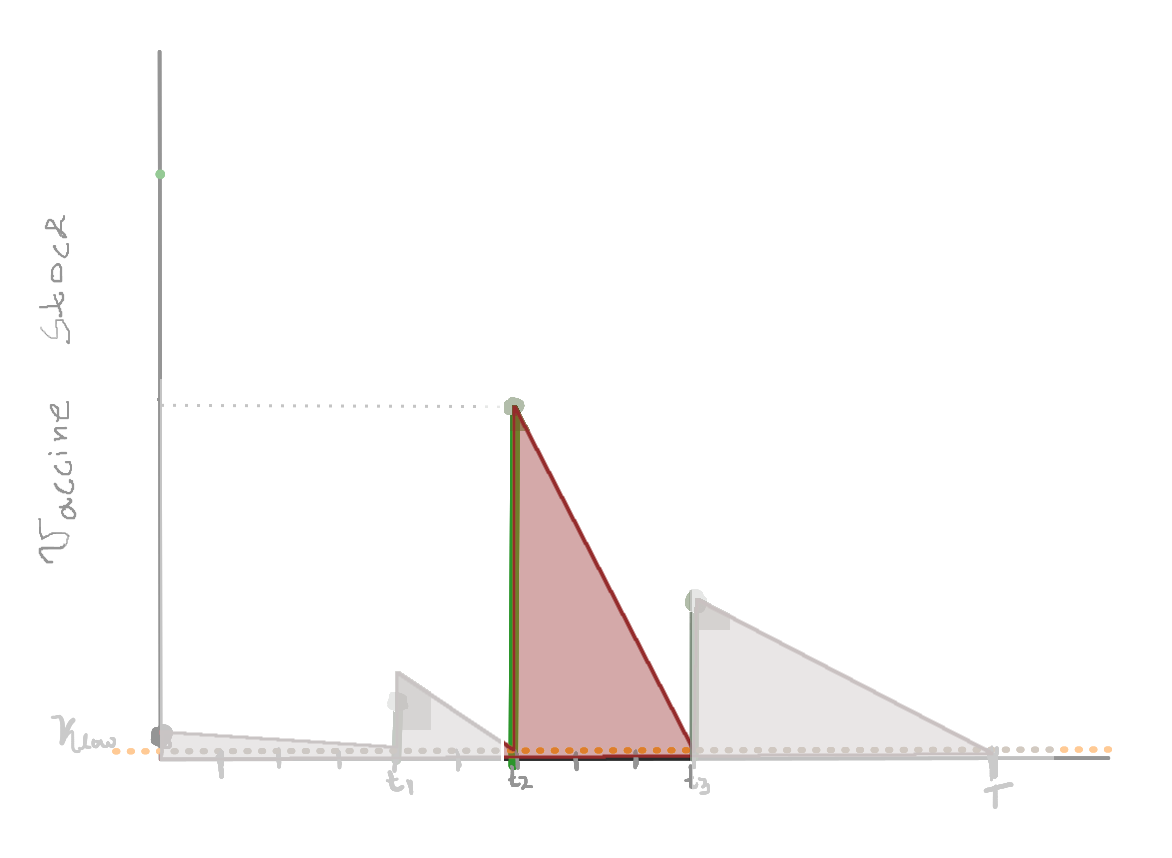
\includegraphics[%
                        width=.7\textwidth,%
                        keepaspectratio=true]{images/Fig01_002_00.png}
                }
%
                \only<6-8>{
                    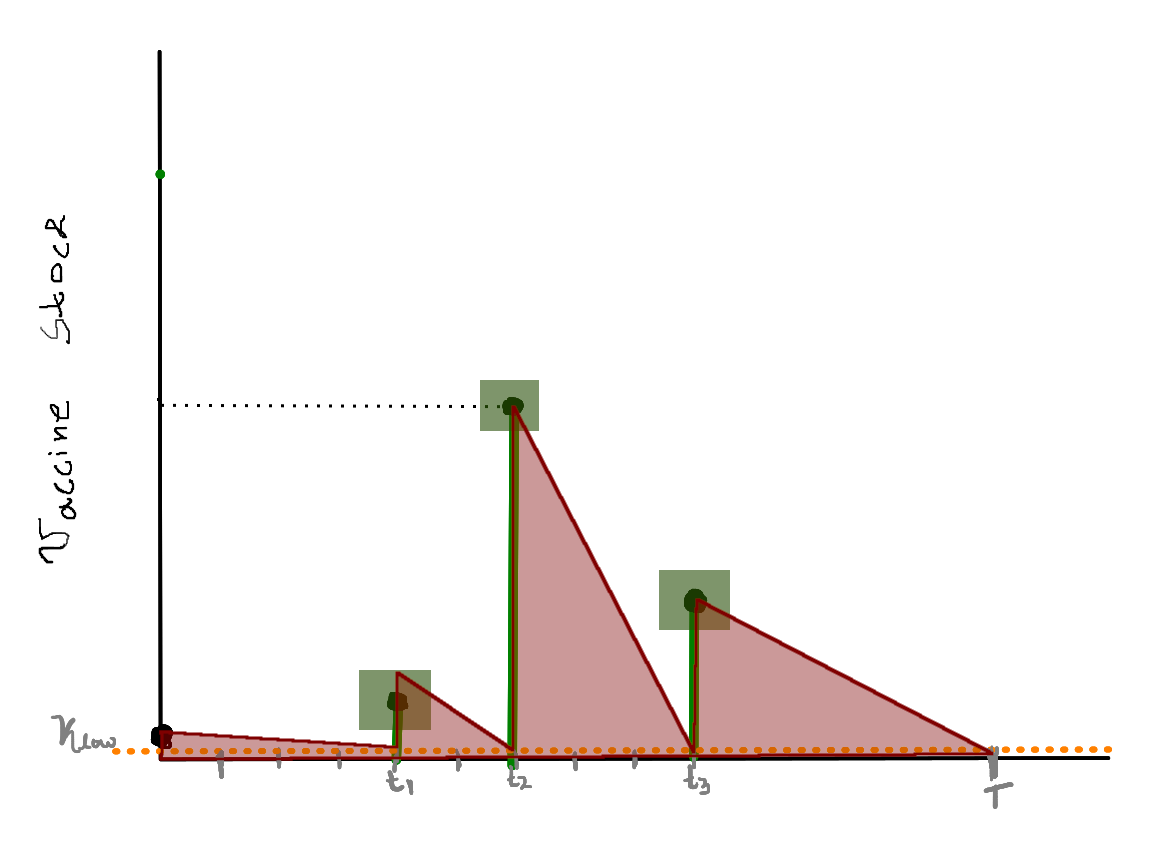
\includegraphics[%
                        width=.7\textwidth,%
                        keepaspectratio=true]{images/Fig01_002.png}
                }
                \only<9>{
                    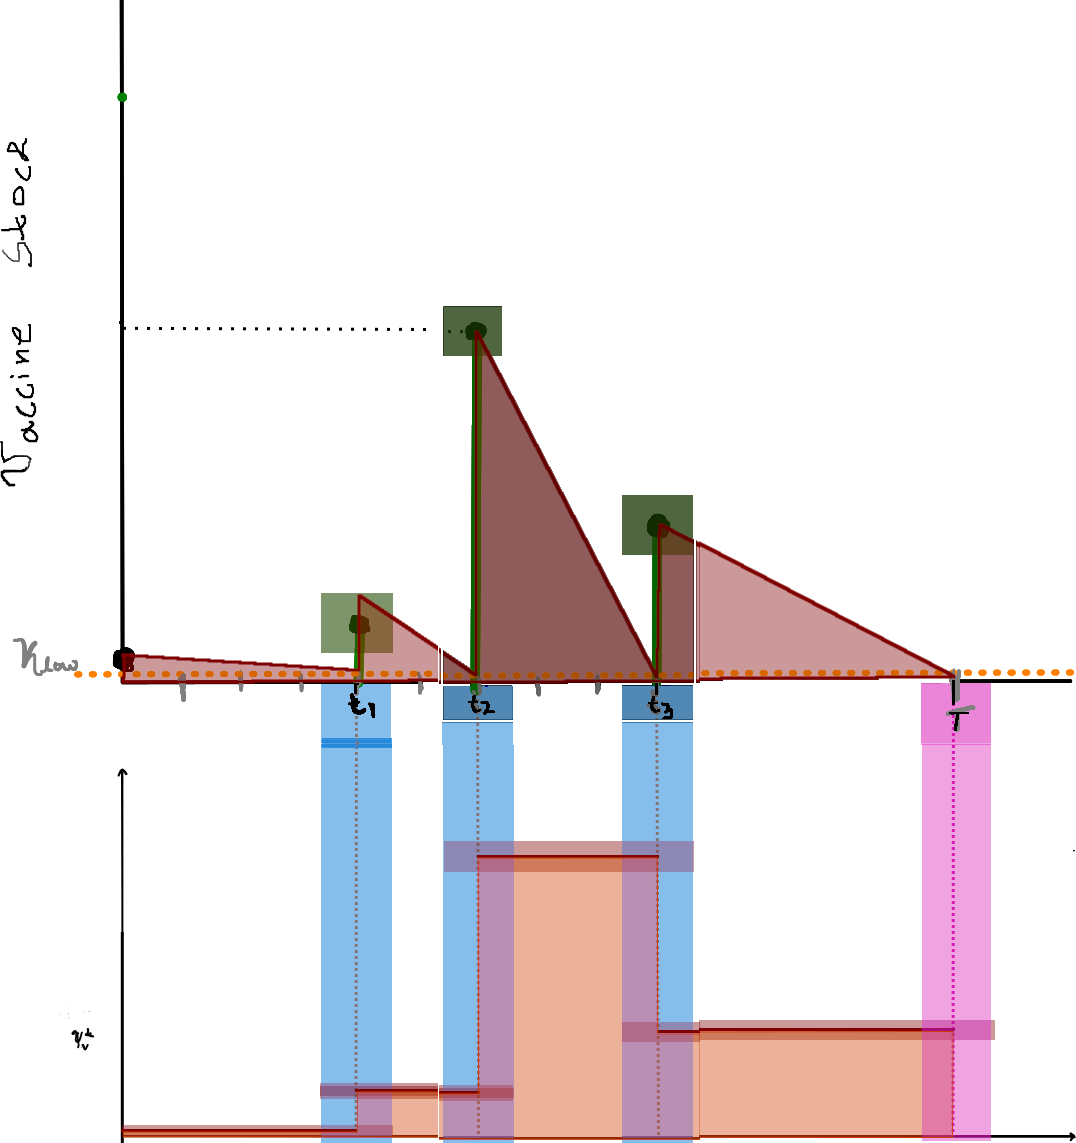
\includegraphics[%
                        width=.65\textwidth,%
                        keepaspectratio=true]{images/Fig01_004_00.png}
                }
                \only<10>{
                    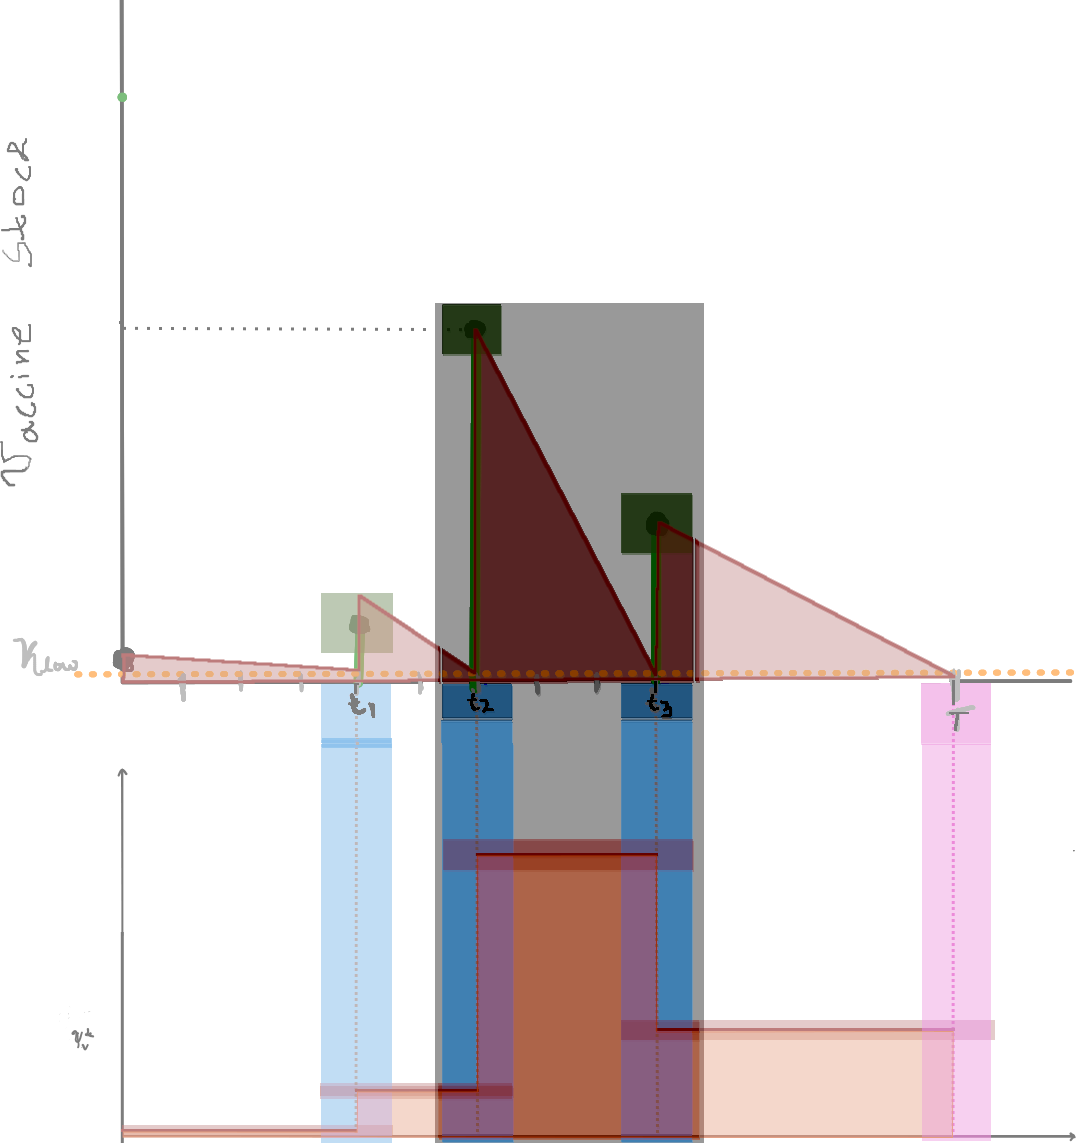
\includegraphics[%
                        width=.65\textwidth,%
                        keepaspectratio=true]{images/Fig01_004_01.png}
                }
                \end{center}
            \end{overlayarea}
        \end{textblock*}
    \begin{textblock*}{120mm}(0mm,57mm)
        \begin{center}
            \only<5-6>{
                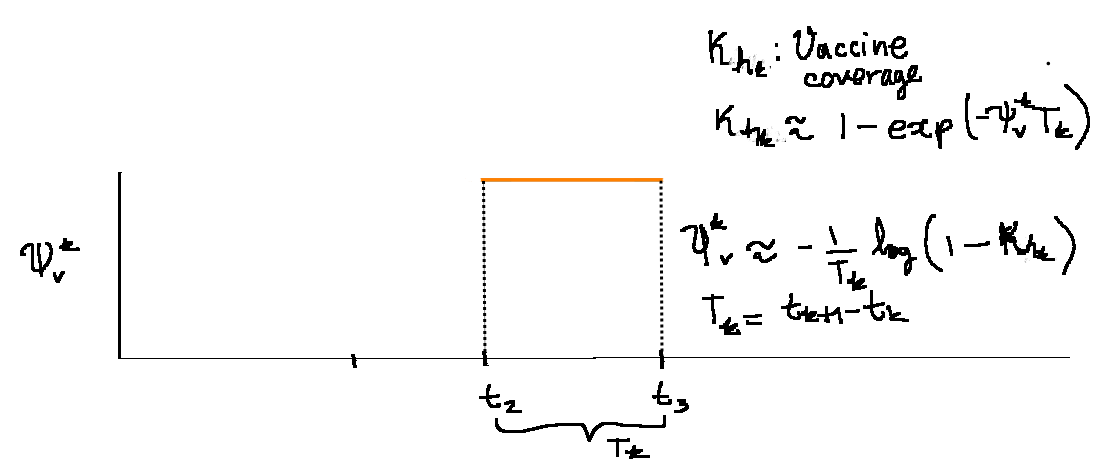
\includegraphics[%
                        width=0.65\textwidth,%
                        keepaspectratio=true]{images/Fig01_002_01.png}
            }
            \only<7>{
                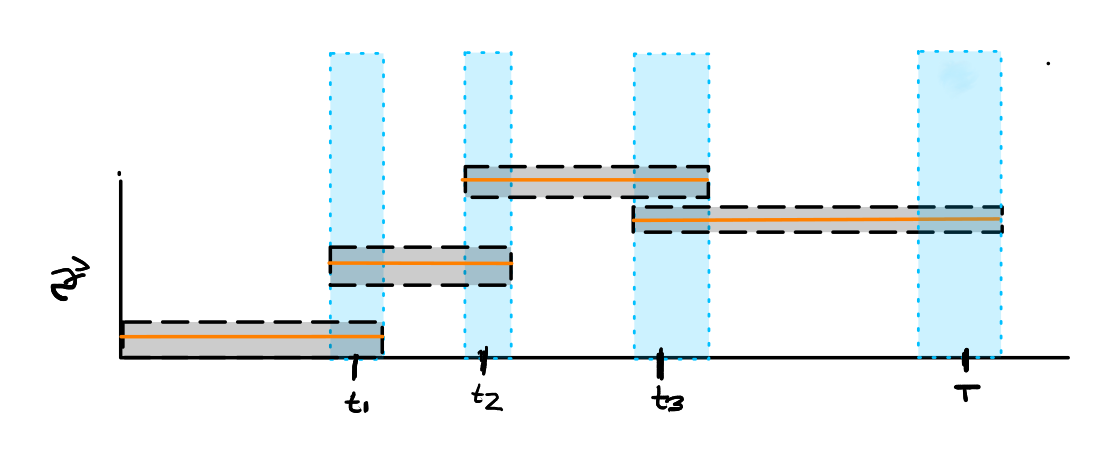
\includegraphics[%
                        width=0.65\textwidth,%
                        keepaspectratio=true]{images/Fig01_002_02.png}
            }
            \only<8>{
                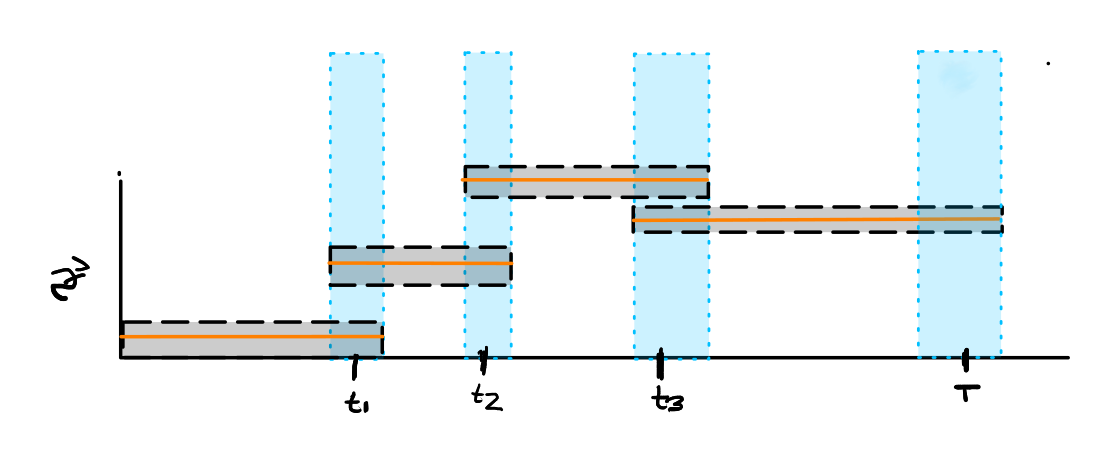
\includegraphics[%
                    width=.65\textwidth,%
                    keepaspectratio=true]{images/Fig01_003.png}
            }
        \end{center}
    \end{textblock*}
\end{frame}
%%%%%%
\begin{frame}{Model Scheme}
    \setlength{\leftmargini}{1mm}
    %!TEX root = ../main.tex
        \setlength{\leftmargini}{1mm}
        \begin{textblock*}{65mm}(5mm, 12mm)
            \only<1>{
                \includegraphics[scale=0.12,%
                    keepaspectratio]{assets/%
                    SchemeModel_withoutVaccination.png}
            }
            \only<2>{
                \includegraphics[scale=0.12,%
                    keepaspectratio]{assets/%
                    SchemeModel_withoutVaccination00.png}
            }
            \only<3->{
                \includegraphics[scale=0.12,%
                    keepaspectratio]{assets/%
                    SchemeModel_withoutVaccination01.png}
            }
        \end{textblock*}
%
    \begin{textblock*}{45mm}(82mm, 50mm)
        \only<2-4>{
            \begin{bluebox}{Vaccine Hypotheses}
                \begin{itemize}
                    %TODO: change bullet indentation
                    \item
                        Imperfect preventive
                    \item
                        One dose
                    \item
                        Symptomatic exception
                    \item
                        Action over susceptible
                \end{itemize}
            \end{bluebox}
        }
    \end{textblock*}
    \begin{textblock*}{75mm}(5mm, 65mm)
    \only<4->{
        \begin{bluebox}{Notation}
            \begin{tabular}{rl}
                $\epsilon$
                & vaccine efficacy
                \\
                $p$
                & Generation of symptoms  probability
                % \\
                % $u_V(t)$
                % & Optimal vaccination policy
            \end{tabular}
        \end{bluebox}
        }
    \end{textblock*}
%
    \begin{textblock*}{45mm}(82mm, 45mm)
        \only<5->{
            \begin{bluebox}{SAGE objectives}
                \begin{itemize}
                    \item
                        Vaccine profile \\(Efficacy, immunity)
                    \item
                        Coverage
                    \item
                        Time Horizon
                \end{itemize}
                \tcblower
                \only<6->{
                    Immunity:
                    \begin{itemize}
                        \item
                            natural (reinfection)
                        \item
                            vaccine-induced
                    \end{itemize}
                }
            \end{bluebox}
        }
    \end{textblock*}
\end{frame}
% %
\begin{frame}
    \begin{textblock*}{80mm}(-5mm, 8mm)
        \begin{align*}
            \frac{d S}{dt}
                &=
                \mu \widehat{N}
                - (\lambda_f + \mu + \psi_V) S
                + \omega_V V + \delta_R R
            \\
            \frac{d E}{dt}
                &=
                \lambda_f S +
                (1- \epsilon) V - (\mu + \delta_E) E
            \\
            \frac{d I_S}{dt}
            &=
                p \delta_E E - (\mu + \alpha_S) I_S
            \\
            \frac{d I_A}{dt}
            &= (1- p)\delta_E E
                - (\mu + \alpha_A)I_A
            \\
            \frac{d R}{dt}
                &= (1 - \theta) \alpha_S I_S
                + \alpha_A I_A
                -(\mu + \delta_R) R
            \\
            \frac{d D}{dt}
            &=  \theta \alpha_S I_S
            \\
            \frac{d V}{dt}
                &= \psi_V S -
                \left[
                    (1 - \epsilon ) \lambda_f + \mu + \omega _V
                \right] V
            \\
            X_{vac}^{\prime} &= \psi_V (S + E + I_A + R)
            \\
            \widehat{N} &= S +E+ I_A + I_S + R, \quad
            \widehat{N} + D = 1
            \\
            \lambda_f &:= \frac{\beta_S I_S + \beta_A I_A}{\widehat{N}}
            %\psi(h) &= 1 - e^{-h} (1- \psi(h) \mu) I_A^n
        \end{align*}
    \end{textblock*}
\end{frame}

